%%%%%%%%%%%%%%%%%%%%%%%%%%%%%%%%%%%%%%%%%%%%%%%%%%%%%%%%%%%%%%%%%%%%%%%%%%%%%
\section{Dynamic and Irregular Scientific Applications}\label{sec:back-apps}
%%%%%%%%%%%%%%%%%%%%%%%%%%%%%%%%%%%%%%%%%%%%%%%%%%%%%%%%%%%%%%%%%%%%%%%%%%%%%
In this section, we introduce several scientific applications that are
widely used in physics, chemistry and informatics fields. Each of them
performs dynamic computation and always involves extremely large computing
data. To fully utilize advanced HPC systems, computational scientists are
looking at the ways to improve these applications in order to solve larger
problem sizes with highly accurate results.

\subsection{Quantum Monte Carlo Simulation}
Quantum Monte Carlo (QMC) method is one of the most accurate solution to
provide accurate and reliable approximation for quantum many-body systems.
It helps scientists study the complex electronic structure of realistic
world on large-scale computing systems. The algorithm of QMC method is
mainly designed around two data objects: enormous ``walkers'' to represent
the dynamic status of each particle, and a large but read-only ensemble
data that shared among all walkers. The traditional implementation of
QMC method utilizes MPI to distribute the walkers among multiple processes
and simply replicate the ensemble data on each MPI process. However,
such design extremely limits researchers to study larger physical systems
or achieve more accurate simulations since the ensemble data is so large
that always takes Gigabytes memory per core. Especially on modern
mulit- and many-core systems, whose memory capacity per core is actually
reducing, a more efficient design is required.

QMCPACk is an open-source QMC package implemented using hybrid MPI+
threads programming model for massively parallel computing system~\cite{qmcpack}.
It utilizes threads to parallelize the walkers inside every physical node
thus the essential memory restriction can be addressed since the large
enormous data can be shared among threads on every node, and employs MPI
for inter-node communication as demonstrated in Figure~\ref{fig:app-qmcpack}.
This design also benefits from reduced collective communication among
MPI processes that is used for global reduction calculation among walkers,
and from less number of large point-to-point communication between paired
MPI processes for exchanging walker objects in the load balance step.

\begin{figure}[ht]
\centering
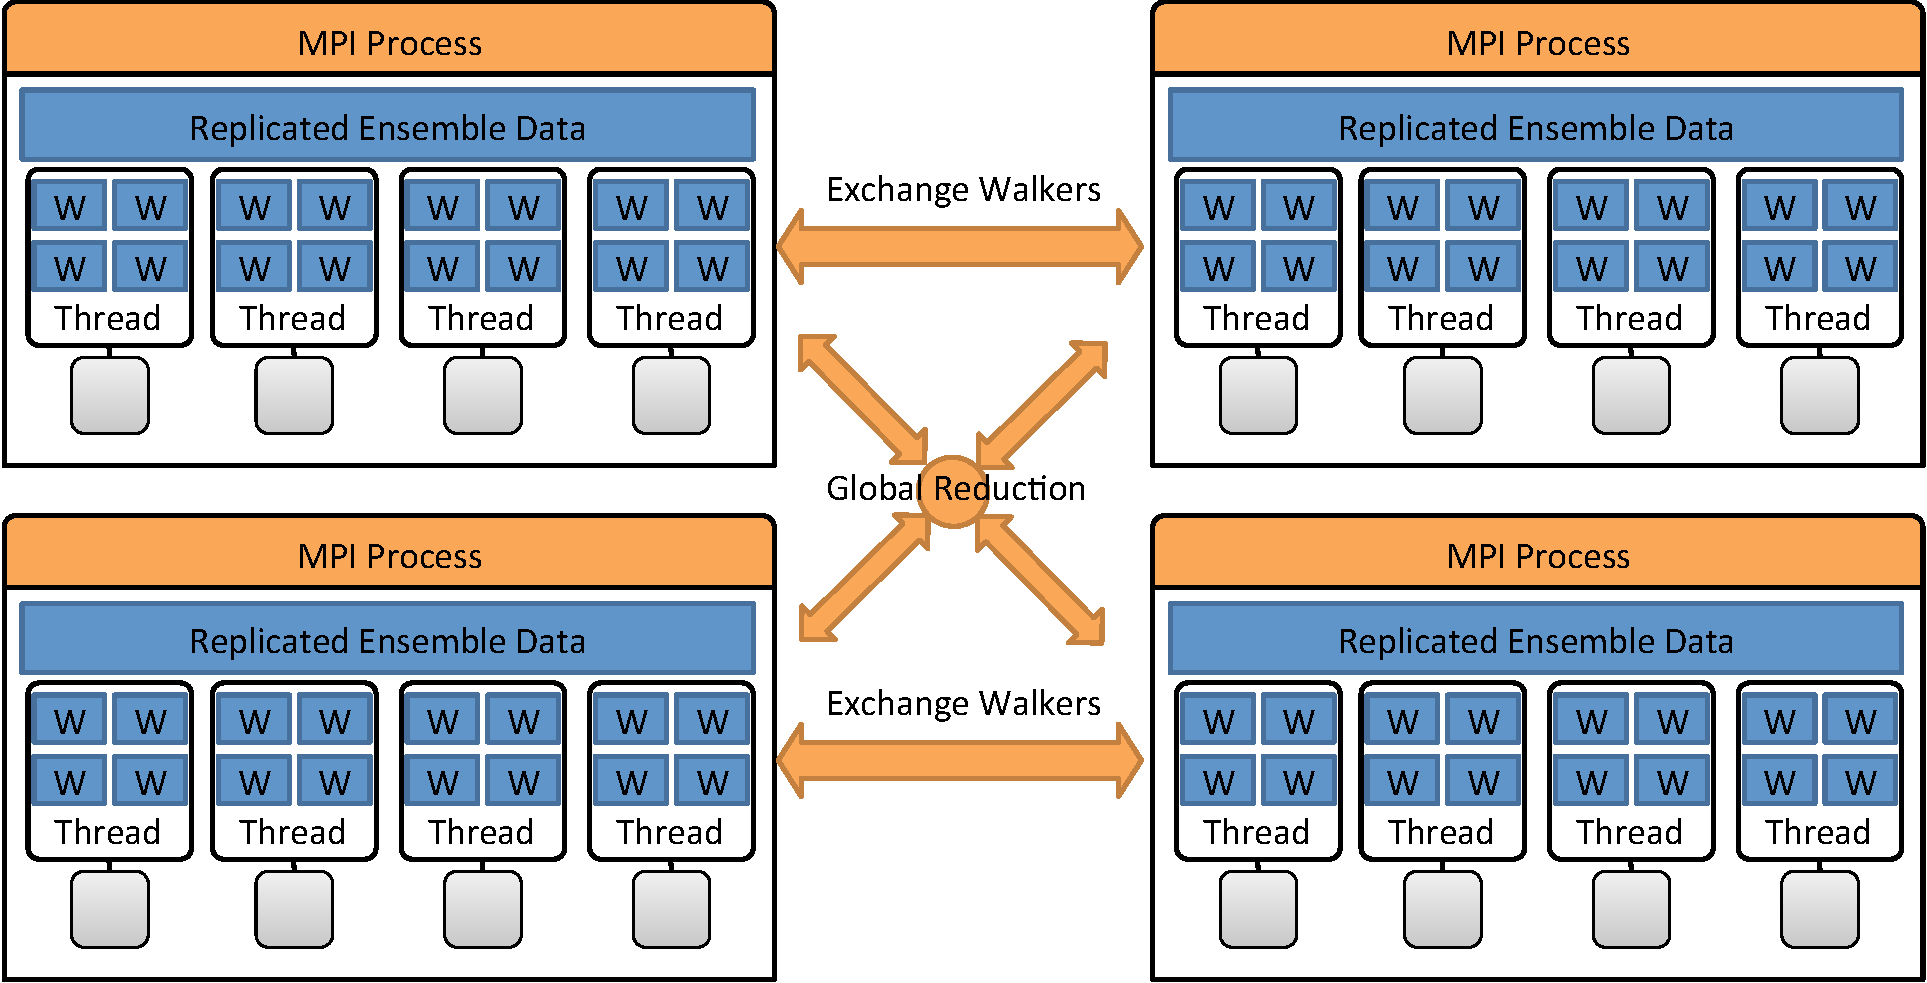
\includegraphics[width=1\textwidth]{figures/background/app-qmcpack.pdf}
\caption{Hybrid Implementation of Quantum Monte Carlo Simulation.}
\label{fig:app-qmcpack}
\end{figure}

\subsection{Computational Fluid Dynamics}
Nek5000 is an open-source code that widely used in a broad range of
applications such as nuclear reactor cores, ocean modeling and combustion
simulation~\cite{nek5000}. It provides high order, incompressible
Navier-Stokes solver based on the spectral element method. The implementation
of Nek5000 is mainly composed of conjugate gradient (CG) solver with
efficient preconditioners, which is captured in the Nekbone mini-application
with the basic structure and user interface.

The main computational kernel of Nekbone consists of multi-grid matrix-matrix
multiplications. Several researches have looked into the optimization for
such computation pattern on advanced heterogeneous HPC architectures. For
example, Markidis et al.~\cite{nek-openacc} presented an MPI+OpenACC version
of Nek5000 code to highly parallelize the most time-consuming ax3D and
gs\_op subroutines on GPU-accelerated systems. Hart and Ivanov et al.'s papers
~\cite{nek-eva, nek-openmp4} have also contributed the OpenMP version of
the Nekbone mini-application for accelerating the local computation on
Cray supercomputers.


\subsection{NWChem Quantum Chemistry Application}
NWChem is a widely used quantum chemistry application suite that provides
a large set of simulation capabilities~\cite{nwchem}. Due to the large
memory needs in NWChem that often require memory sharing across multiple
nodes, it is developed based on the Global Arrays toolkit~\cite{GA_SC94}
which provides users with distributed dense arrays that can be accessed
through one-sided operations. Figure~\ref{fig:app-nwchem-pattern}
demonstrates the typical \emp{get-compute-update} pattern used in NWChem.

Current NWChem has been looking at small-to-medium molecules (e.g.,
(H$_2$O)$_{21}$ as shown in Figure~\ref{fig:app-nwchem-w21}) consisting of
20-100 atoms. Since the coulomb interaction among such small amount of
atoms is reasonably large, the computation and communication can be
successful scaled on modern supercomputers. However, scientists aim to
study more complex molecules that are composed of thousands atoms or even
larger thus not only the short-range interactions but also the long-range
interactions have to be covered. This means, the diversity of the amount
of computation per process can be considerably increased, thus resulting
in extremely irregular computation with data movement.

\begin{figure}[ht]
\centering
\subfigure[Interaction in (H$_2$O)$_{21}$ molecule.] {
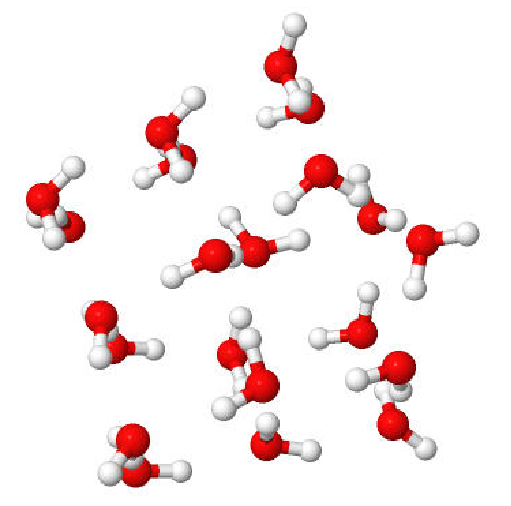
\includegraphics[width=0.38\textwidth]{figures/background/app-nwchem-w21.pdf}
\label{fig:app-nwchem-w21}}
\subfigure[Get-Compute-Update pattern.] {
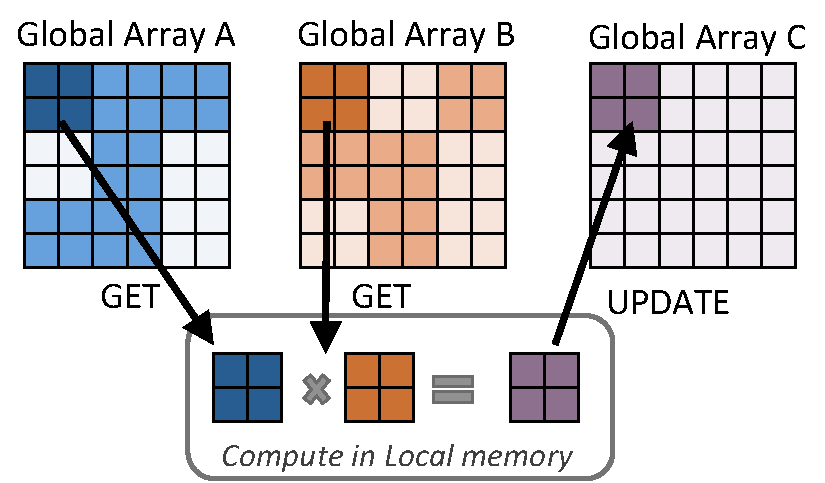
\includegraphics[width=0.56\textwidth]{figures/background/app-nwchem-get-comp-update.pdf}
\label{fig:app-nwchem-pattern}}
\caption{Communication in NWChem Application.}
\label{fig:app-nwchem}
% \vspace{-2.0ex}
\end{figure}


\subsection{SWAP-Assembly Bionformatics Application}

In bioinformatics, since it is still hard to read the whole genomes
in modern DNA sequencing technology, researchers often break down long
DNA samples into large amount of small fragments, called ``reads'', and
then read those reads into digital data as the first step. The next step
is called assembly, which merges overlapping reads back to one or several
contiguous DNA sequences. The sequence assembly technology helps biology
scientists analyze DNA sequence, and is especially important for understanding
complex environments containing many different microbiomes (e.g., soil and
seawater).

The SWAP-Assembler software provides highly scalable assembler that processes
the sequence assembly on thousands of cores in parallel~\cite{swap}. The
initial reads are represented as a distributed De Bruijn graph (e.g., )
Figure~\ref{fig:app-swap-graph}), and final contiguous DNA chains are
assembled by executing multiple rounds of graph reduction and error removal
over MPI communication. The communication pattern follows the
\emp{send-merge-return} mode as shown in Figure~\ref{fig:app-swap-merge}.
Every process issues each of its local DNA read to a remote process to find
the overlapping reads. On the remote process, it first searches the
overlapping read for every received message, then merges the reads and
finally returns the merged result. If there is no matching read on the
remote side, the sending process will try another remote process following
the same patter. This processing always involves enormous irregular data
movement over petabytes of data and requires several days or even months of
computation. For instance, the largest simulation done to date was at the
University of Chicago, where a 2.3-terabyte sample was assembled on a
supercomputer with 18,000 cores—this simulation took 4 days to complete and
spent 99.9\% of its time idling, because of imbalance between processing
units.


\begin{figure}[ht]
\centering
\subfigure[Graph Reduction.] {
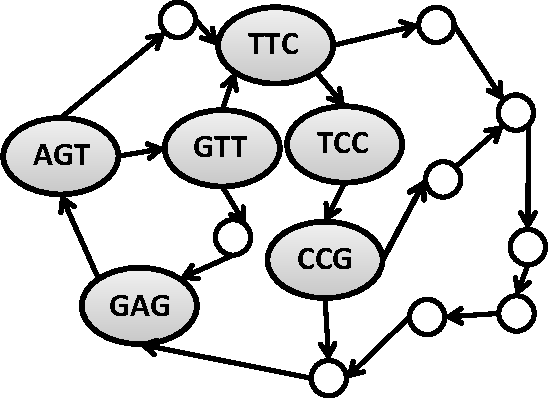
\includegraphics[width=0.3\textwidth]{figures/background/app-swap-graph.pdf}
\label{fig:app-swap-graph}}
\subfigure[Communication Pattern.] {
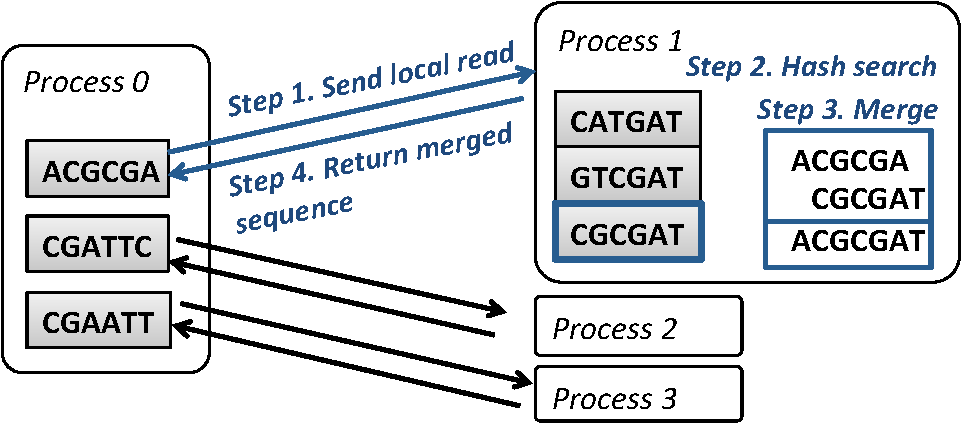
\includegraphics[width=0.65\textwidth]{figures/background/app-swap-merge.pdf}
\label{fig:app-swap-merge}}
% \includegraphics[width=0.9\columnwidth]{figures/background/swap-merge.pdf}
\caption{Irregular Communication in SWAP-Assembly.}
\label{fig:app-swap}
% \vspace{-2.0ex}
\end{figure}

% \subsection{Nuclear Reactor Core Modeling}
% \subsection{Graph-Type Parallel Visualization}

\subsection{Green’s Function Monte Carlo}

Green’s Function Monte Carlo (GFMC) is an application in theoretical nuclear
physics that provides ab initio calculations for few-nucleon systems~\cite{gfmc}.
It describes the nuclear structures and reactions by solving the
Schr\"{o}dinger equation and is recognized as the most reliable method
for nuclei with 12 or fewer nucleons. The implementation of GFMC utilizes
OpenMP to parallelize heavy sparse matrix-vector multiplications and
uses MPI to communicate among distributed computing nodes.

The Asynchronous Dynamic Load Balancing (ADLB) library~\cite{adlb} is
essentially designed for addressing the load balancing among MPI processes
in GFMC on large scale systems that contain more than one hundred thousand
computing cores. It provides a general-purpose worker-server model with
one-sided Put/Get operations that helps application codes dynamical
share work tasks with assorted work types and priorities. A few server
processes are initialized to maintain a distributed shared work queue.
Application processes can then submit arbitrary work tasks to the queue
with necessary data, and retrieve the results after any task is finished.
